\documentclass{training}
\schoollogo{../../resources/intros/UI-01-atomic-design.jpg}
\newcommand{\uxfond}{../../resources/fond/UI-01-atomic-design.png}
% Filigrane PAR MODULE : \uxfond (PNG A4 dilue 30 %). Cadre noir vectoriel commun.
% Proportions original 744 px : marge 20/744, trait 1/744. Exterieur BLANC.
% Cadre via eso-pic +\put (coordonnees absolues) — pas de remember picture (decalage).
\usepackage{eso-pic}

\providecommand{\uxfond}{../../resources/fond/norme_fond_paliers_30.png}

\newlength{\uxmargin}
\newlength{\uxthick}
\newlength{\uxinnerw}
\newlength{\uxinnerh}
\setlength{\uxmargin}{0.02688\paperwidth}% 20/744
\setlength{\uxthick}{0.001344\paperwidth}% 1/744
\setlength{\uxinnerw}{\dimexpr\paperwidth-2\uxmargin-2\uxthick\relax}
\setlength{\uxinnerh}{\dimexpr\paperheight-2\uxmargin-2\uxthick\relax}

% Contenu strictement a l'interieur du trait (+ jour confortable).
\geometry{%
  includeheadfoot,
  left=22mm,
  right=22mm,
  top=20mm,
  bottom=18mm,
  headheight=30pt,
  headsep=5mm,
  footskip=12mm%
}

\AddToShipoutPictureBG{%
  \AtPageLowerLeft{%
    % Fond blanc page entiere
    \put(0,0){\color{white}\rule{\paperwidth}{\paperheight}}%
    % Filigrane module a l'interieur du cadre
    \put(\LenToUnit{\dimexpr\uxmargin+\uxthick\relax},\LenToUnit{\dimexpr\uxmargin+\uxthick\relax}){%
      \includegraphics[width=\uxinnerw,height=\uxinnerh]{\uxfond}}%
    % Cadre noir : bas, haut, gauche, droite
    \put(\LenToUnit{\uxmargin},\LenToUnit{\uxmargin}){%
      \color{black}\rule{\dimexpr\paperwidth-2\uxmargin\relax}{\uxthick}}%
    \put(\LenToUnit{\uxmargin},\LenToUnit{\dimexpr\paperheight-\uxmargin-\uxthick\relax}){%
      \color{black}\rule{\dimexpr\paperwidth-2\uxmargin\relax}{\uxthick}}%
    \put(\LenToUnit{\uxmargin},\LenToUnit{\uxmargin}){%
      \color{black}\rule{\uxthick}{\dimexpr\paperheight-2\uxmargin\relax}}%
    \put(\LenToUnit{\dimexpr\paperwidth-\uxmargin-\uxthick\relax},\LenToUnit{\uxmargin}){%
      \color{black}\rule{\uxthick}{\dimexpr\paperheight-2\uxmargin\relax}}%
  }%
}

\makeatletter
\fancyhf{}
\fancyheadoffset{0pt}
\renewcommand{\headrulewidth}{0pt}
\lhead{\parbox[t]{0.56\textwidth}{\RaggedRight\footnotesize\sloppy\@title}}
\rhead{\parbox[t]{0.36\textwidth}{\RaggedLeft\footnotesize\sloppy\@subtitle}}
\cfoot{\thepage}
% Coupures : underscore et slash dans les noms de fichiers / consignes
\DeclareRobustCommand{\_}{\textunderscore\allowbreak}
\makeatother

% Evite les depassements de longues lignes (Github, Name_FirstName_...)
\sloppy
\emergencystretch=3em
\hbadness=10000

% Sommaire type 42 : chapitres seulement
\setcounter{tocdepth}{0}
\renewcommand{\cftchappresnum}{}
\renewcommand{\cftchapaftersnum}{}
\setlength{\cftchapnumwidth}{2.0em}
\setlength{\cftbeforechapskip}{0.35em}
\cftsetindents{chapter}{0em}{2.0em}


\begin{document}

\title{Atomic design}
\subtitle{Piscine UX/UI --- UI}
\member{Piscine UX/UI}{https://github.com/01-edu/UX-UI}
\summary{From a browse of systems to two libraries with a job.}
\version{1.0}
\prerequisite{The previous module of this piscine, or none if this is your first.}
\maketitle

\newpage
\tableofcontents
\newpage


\chapter{Instructions}

The foreword is not an exercise. It will not be graded. The exercises start at the next chapter, from the easiest contract to the hardest. A later exercise is not taken into account if an earlier one does not hold.

Only what is in the turn-in directory of an exercise is looked at. Do not add files that the exercise does not name. The name of a deliverable follows the pattern in the exercise: \texttt{Name\_FirstName\_DeliverableName\_Date\_VersionNumber}.

You will not be given the gesture. The examples in an exercise sometimes carry a constraint that the sentence does not repeat. Read them. Your other references are the manual of the tool you picked, the person sitting next to you, and the links printed in the exercise.

The order is the order of the quest. Skipping a step because a later screen looks more interesting produces a screen nobody can explain.

\subsection*{About the pictures}

The mark on the cover is the picture of this module. The pale steps behind the text are the page ground. Neither one is a hint.

\subsection*{About machines that write}

You may use a tool to look up a term, the way you would use a dictionary. You may not replace an interview, a test, or a file with a generated text and sign it. If you cannot point at the person, the screen, or the line you claim, the exercise is not done.


\chapter{Foreword}

Brad Frost named the ladder atom, molecule, organism, template, page, and put the essay online (\url{https://atomicdesign.bradfrost.com/}). It is a vocabulary, the way a manual page is a vocabulary. Naming a button an atom does not design the library.

\begin{center}
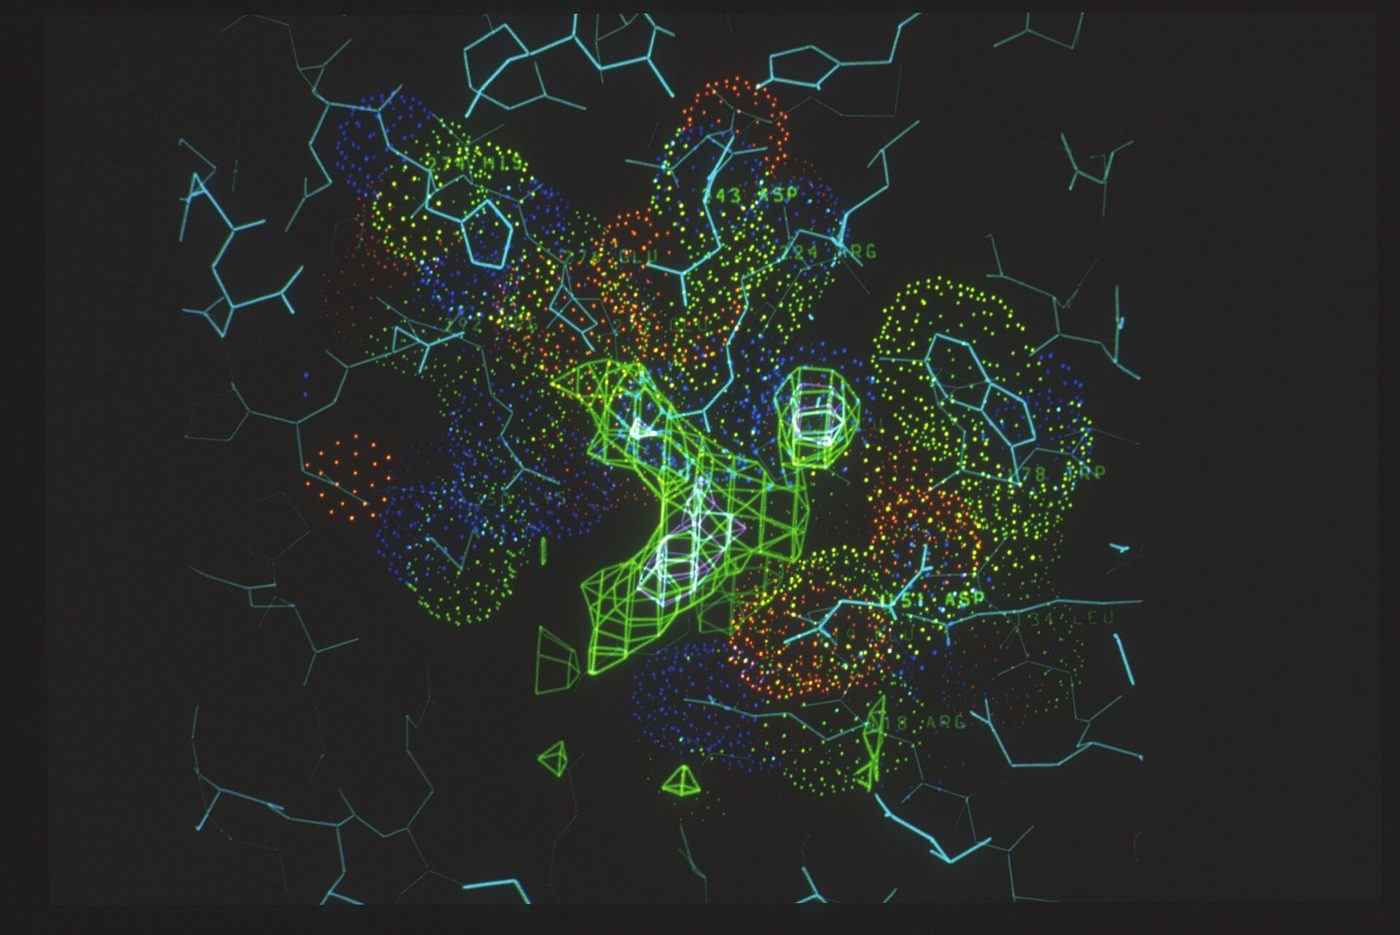
\includegraphics[width=0.78\textwidth,height=0.32\textheight,keepaspectratio]{../../resources/intros/UI-01-atomic-design.jpg}\\[0.4em]
{\footnotesize Picture: division, CSIRO, CC BY 3.0}
\end{center}

Recommended watching. The videos are context. They are not the deliverable.
\begin{itemize}
\item UI - Introduction \& Quest n°1, 01Edu \url{https://www.youtube.com/watch?v=UbE6WMeuvQg&list=PLHyAJ_GrRtf-_aBft2jQL4-QAunn2bLvu}
\end{itemize}

\chapter{Exercise 00: UI II - Ex 1 - Browsing}
\exnumber{00}
\extitle{UI II - Ex 1 - Browsing}
\exfiles{ex00/Figma file, named Name\_FirstName\_DeliverableName\_Date\_VersionNumber}
\exauthorize{Those named in the exercise}
\makeheaderfiles

\textbf{Context:}

Welcome to the 2nd quest of UI!

This series of exercises is a great occasion for you to discover how libraries are made in UI, thanks to Atomic Design.

\textbf{Instructions:}

Among these 4 websites, make snapshots of these elements:

\begin{itemize}
\item 1 template
\item 1 organism
\item 1 molecule
\item 1 atom
\end{itemize}

\textbf{Websites:}

\begin{itemize}
\item Alibaba
\item Booking.com
\item Easyjet App
\item Interrail
\end{itemize}

\textbf{Deliverables:}

\begin{itemize}
\item A Figma file of 4 pages
\item On each page, a screenshot of a template, an organism, a molecule and an atom
\item Upload the Figma file on Github, labeled as follows: "Name\_FirstName\_DeliverableName\_Date\_VersionNumber". For example, it can be labeled as "Doe\_John\_MidFiPrototype\_05242024\_V1".
\item Add a title within the file.
\item Pay attention to the global aspect of the file. It must be clear, simple and easy to read. You can get inspiration on canva.com but don't overload your design with too much details!
\end{itemize}

\textbf{Resources:}

\begin{itemize}
\item Atomic Design Methodology \url{https://atomicdesign.bradfrost.com/chapter-2/}
\item Video tutorial on Figma \url{https://www.youtube.com/watch?v=FTFaQWZBqQ8}
\item Beginning graphic design \url{https://edu.gcfglobal.org/en/beginning-graphic-design/}
\item Gareth graphic studio \url{https://www.youtube.com/c/GarethDavidStudio}
\item Example here \url{https://www.figma.com/file/fzqDkk8Zc8qJCiSMbKV0Ei/UI-II---Ex-1?node-id=0%3A1}
\end{itemize}

\textbf{Quote:}

\begin{itemize}
\item User Interface Design is a hybrid role and can bring together concepts from interaction design, visual design, information architecture and even Front End Development
\end{itemize}


\chapter{Exercise 01: UI II - Ex 2 - Material Design}
\exnumber{01}
\extitle{UI II - Ex 2 - Material Design}
\exfiles{ex01/Figma file, named Name\_FirstName\_DeliverableName\_Date\_VersionNumber}
\exauthorize{Those named in the exercise}
\makeheaderfiles

\textbf{Instructions:}

Download this image \url{https://storage.googleapis.com/gd-wagtail-prod-assets/original_images/MDA2018_inline_02.jpg} which is a snapshot of 3 screens of Lyft, and detect the order in which the layers were set.

\textbf{Deliverables:}

\begin{itemize}
\item A Figma file with the image
\item On each screen, indicate the layers order with numbers. 1 being the background image, 2 the element right on top, etc.
\item Upload the Figma file on Github, labeled as follows: "Name\_FirstName\_DeliverableName\_Date\_VersionNumber". For example, it can be labeled as "Doe\_John\_MidFiPrototype\_05242024\_V1".
\item Add a title within the file.
\item Pay attention to the global aspect of the file. It must be clear, simple and easy to read. You can get inspiration on canva.com but don't overload your design with too much details!
\end{itemize}

\textbf{Tips:}

\begin{itemize}
\item 2 numbers can be switched as long as the layering of layers is respected 
\end{itemize}

\textbf{Resources:}

\begin{itemize}
\item Material Design Awards 2019 \url{https://design.google/library/material-design-awards-2019/}
\item What is Material Design - Wikipedia \url{https://en.wikipedia.org/wiki/Material_Design}
\end{itemize}


\chapter{Exercise 02: UI II - Ex 3 - Design system library}
\exnumber{02}
\extitle{UI II - Ex 3 - Design system library}
\exfiles{ex02/Figma file, named Name\_FirstName\_DeliverableName\_Date\_VersionNumber}
\exauthorize{Those named in the exercise}
\makeheaderfiles

\textbf{Instructions:}

Copy 10 elements from easyJet design system, including

\begin{itemize}
\item atoms
\item molecules
\item organisms
\end{itemize}

\textbf{Deliverable:}

\begin{itemize}
\item A Figma file including 10 elements from easyJet design system
\item Upload the Figma file on Github, labeled as follows: "Name\_FirstName\_DeliverableName\_Date\_VersionNumber". For example, it can be labeled as "Doe\_John\_MidFiPrototype\_05242024\_V1".
\item Add a title within the file.
\item Pay attention to the global aspect of the file. It must be clear, simple and easy to read. You can get inspiration on canva.com but don't overload your design with too much details!
\end{itemize}

\textbf{Tips:}

\begin{itemize}
\item You can use Avenir Book instead of easyJet's font
\item Explore Noun Project to get icons
\end{itemize}

\textbf{Resources:}

\begin{itemize}
\item Atomic Design Methodology \url{https://atomicdesign.bradfrost.com/chapter-2/} 
\end{itemize}


\chapter{Exercise 03: UI II - Ex 4 - Library for climbing addicts}
\exnumber{03}
\extitle{UI II - Ex 4 - Library for climbing addicts}
\exfiles{ex03/Figma file, named Name\_FirstName\_DeliverableName\_Date\_VersionNumber}
\exauthorize{Those named in the exercise}
\makeheaderfiles

\textbf{Instructions:}

You are part of a climbing group and volunteer to rebrand the website of your club.

Based on a moodboard, create a design system with at least 20 elements, including atoms, molecules and organisms, and include multistates.

\textbf{Deliverables:}

\begin{itemize}
\item A Figma file with a moodboard for a climbing group. Include:
\begin{itemize}
\item Pictures
\item Colors (2 to 3 main colors)
\item Typography
\end{itemize}
\item A Figma file with a library including:
\begin{itemize}
\item At least graphic design 20 elements
\item At least one atom
\item At least one molecule
\item At least one organism
\item At least 5 multistate elements
\end{itemize}
\item Upload the documents on Github, in a zip folder named "ProjectTitle\_Name\_FirstName", with all project deliverables as follows: "Name\_FirstName\_DeliverableName\_Date\_VersionNumber".  For example, the first deliverable can be named as "Doe\_John\_MidFiPrototype\_05242024\_V1".
\item Add a title within all written documents.
\item Pay attention to the global aspect of the deliverables. They must be clear, simple and easy to read. You can get inspiration on canva.com but don't overload your design with too much details!
\end{itemize}

\textbf{Tips:}

\begin{itemize}
\item Let's be creative! Get inspiration from visuals before diving in.
\item Feel free to get inspiration from existing design systems. Browse Dribble and the Figma community!
\end{itemize}

\textbf{Resources:}

\begin{itemize}
\item Introduction to design systems \url{https://www.youtube.com/watch?v=xEuBCUngJ_U}
\item Create a design system - Figma course \url{https://www.youtube.com/watch?v=RYDiDpW2VkM}
\item Building a design system library - Lyft \url{https://medium.com/tap-to-dismiss/building-a-design-system-library-532ef2492811}
\item Examples of UI Buttons library \url{https://www.pinterest.co.kr/pin/663014376380850291/}
\end{itemize}


\chapter{Exercise 04: UI II - Ex 5 - Library for a dating app}
\exnumber{04}
\extitle{UI II - Ex 5 - Library for a dating app}
\exfiles{ex04/Figma file, named Name\_FirstName\_DeliverableName\_Date\_VersionNumber}
\exauthorize{Those named in the exercise}
\makeheaderfiles

\textbf{Instructions:}

You are asked to design a dating app.

Based on a moodboard you have composed, create a design system with at least 20 elements, including atoms, molecules and organisms, and include multistates.

\textbf{Deliverables:}

\begin{itemize}
\item A Figma file with a moodboard for a dating app. Include:
\begin{itemize}
\item Pictures
\item Colors (2 to 3 main colors)
\item Typography
\end{itemize}
\item A Figma file with a library including
\begin{itemize}
\item At least graphic design 20 elements
\item At least one atom
\item At least one molecule
\item At least one organism
\item At least 5 multistate elements
\end{itemize}
\item Upload the documents on Github, in a zip folder named "ProjectTitle\_Name\_FirstName", with all project deliverables as follows: "Name\_FirstName\_DeliverableName\_Date\_VersionNumber".  For example, the first deliverable can be named as "Doe\_John\_MidFiPrototype\_05242024\_V1".
\item Add a title within all written documents.
\item Pay attention to the global aspect of the deliverables. They must be clear, simple and easy to read. You can get inspiration on canva.com but don't overload your design with too much details!
\end{itemize}

\textbf{Tips:}

\begin{itemize}
\item Let's be creative! Get inspiration from visuals before diving in.
\item Feel free to get inspiration from existing design systems. Browse Dribble and the Figma community!
\end{itemize}

\textbf{Resources:}

\begin{itemize}
\item Introduction to design systems \url{https://www.youtube.com/watch?v=xEuBCUngJ_U}
\item Create a design system - Figma course \url{https://www.youtube.com/watch?v=RYDiDpW2VkM}
\item Building a design system library - Lyft \url{https://medium.com/tap-to-dismiss/building-a-design-system-library-532ef2492811}
\item Examples of UI Buttons library \url{https://www.pinterest.co.kr/pin/663014376380850291/}
\end{itemize}


\end{document}
